%% RESULTS

In this section we present the experiments we will conduct. Two different tracking tasks in presence of external contacts will be investigated.
First, we will demonstrate that a controller using a learned inverse dynamics model can be used to compensate for contact forces and that the tracking performance of a tracking controller will be improved.
In a second experiment, we will demonstrate that the same inverse dynamics model can also be used to avoid an obstacle and gently slide along it. 



\subsection{Experimental Setting}
\label{sec:results:setup}
	Both experimental evaluations are performed on a real \robot{} humanoid robot~\cite{Natale2013}.
    The \robot{} possess 53 degrees of freedom and is 104 cm tall for 24 kg of weight.
    Four 6-axis force/torque sensors placed are proximally in the middle of legs and arms.
    Additionally, artificial skin consisting of more than 2000 tactile sensors are mounted on the robot covers~\cite{Cannata2008}.
 	%
    In our experiments, we control 5 DoF of the \robot{} arm: shoulder pitch, roll and jaw, elbow and wrist pronosupination. 
    Therefore $\q \in \R^5$, $\dq \in \R^5$, $\ddq \in \R^5$, $\torques \in \R^5$ and $\ftsForces \in \R^3$ resulting in learning the mapping $\inputMatrix \in \R^{18} \mapsto \outputMatrix \in \R^5$.
    The skin input~$\skinInput$ from the forearm consists of 270 sensors.
    

	%The information from these three types of sensors is used to estimate the joint torques and the external contact forces by the \idyn{}  library~\cite{Ivaldi2011}. 
	%In the following,  $\torques_{\rm IDYN}$ denotes the joint torques estimated by the \idyn{} library, which we use as a comparison. 
	%For more detail on the contact detection and taxels calibration we refer to~\cite{DelPrete2011,DelPrete2012}.
	%\comment{Still missing the explanation about why iDyn with multiple contacts is bad}

%	These sensors are used to detect the contacts, compute the external contact forces and estimate the joint torques~\cite{Fumagalli2012}. 
%	The tactile elements in the skin (see \fig\ref{fig:icubskin}) provide the information about the contact location; they also provide an indirect measure of the external force. 
%	The force/torque sensors, placed proximally in the middle of legs and arms, are used to estimate the robot dynamics (internal/external wrenches) and the joint torques.
%	This estimation is performed online by the library iDyn, which relies on the known dynamic model of the robot~\cite{Ivaldi2011}. 
%	\comment{Discuss the assumptions of the analytic model: ellipsoid thing}



%===============================================================================

\subsection{Pushing Obstacles}
\label{sec:results:exp1}

	%
    \begin{wrapfigure}{r}{0.2\columnwidth}
	%\begin{figure}[t]
		\centering
		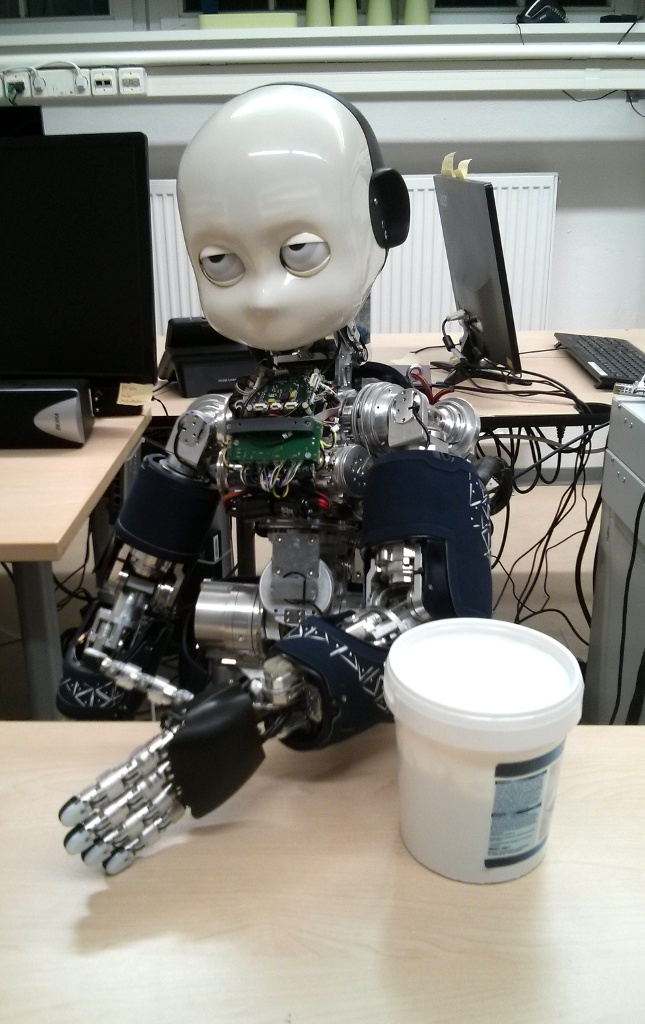
\includegraphics[width=.99\linewidth]{robertoIROS/fig/taskPush}
		\caption{\textbf{\nameref{sec:results:exp1}. }}
		\label{fig:pushSetup}
	%\end{figure}
    \end{wrapfigure}
	%

    For classical controllers, when an obstruction occur, the rigid body inverse dynamics does not account for this variation. 
    As a result, the tracking error increase and the contribution of the PD feedback controller increases to compensate for this tracking error.
	In this scenario we demonstrate that it is possible to use a learned model to improve the tracking accuracy when unforeseen and unknown obstruction are encountered along the path.
    Additionally, we show that such learned dynamics allows to reduce the PD gains to achieve an increased safety, without loss in tracking accuracy.
	
    We first consider the \robot{} following a pre-defined trajectory with the left arm.
    Following, we repeat the same trajectory, but this time with an unforeseen obstruction. 
    
   
% 	%
% 	\begin{figure}[t]
% 		\centering
%         \begin{subfigure}[t]{0.31\hsize}
% 			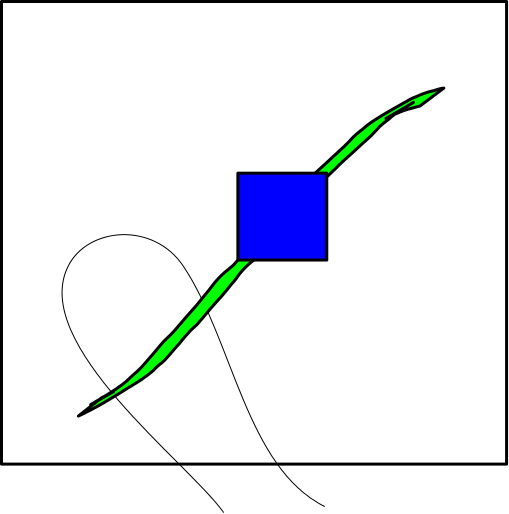
\includegraphics[width=.98\columnwidth]{fig/table_push_01}
%             \caption{Inverse dynamics}
%         \end{subfigure}
%         \hfill
% 		\begin{subfigure}[t]{0.31\hsize}
%         	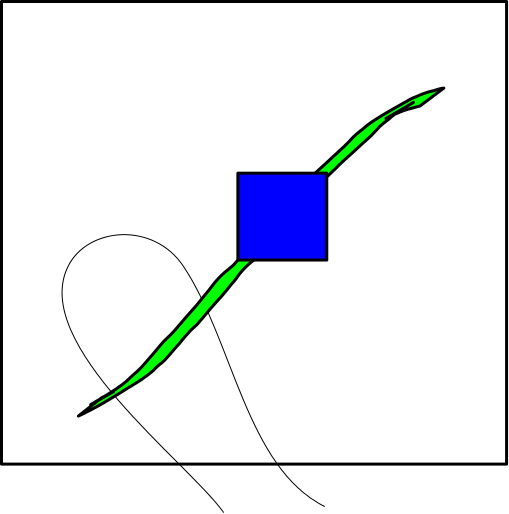
\includegraphics[width=.98\columnwidth]{fig/table_push_01}
%             \caption{iDyn}
%         \end{subfigure}
%         \hfill
%         \begin{subfigure}[t]{0.31\hsize}
% 			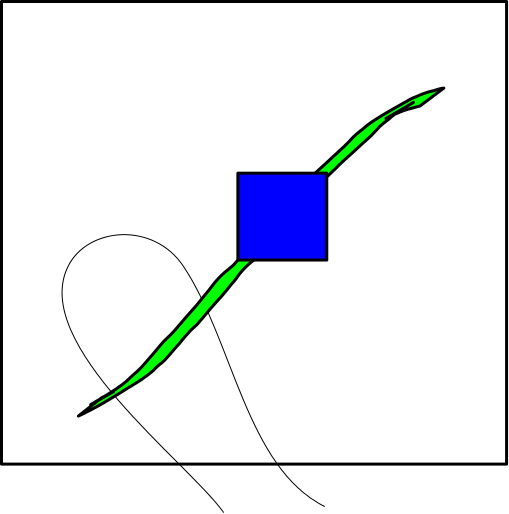
\includegraphics[width=.98\columnwidth]{fig/table_push_01}
%             \caption{Learned inverse dynamics with contacts}
%         \end{subfigure}
% 		\caption{\textbf{\nameref{sec:results:exp1}:} Tracking performance when pushing an obstacle. \textit{on the left}: the performance of the inverse dynamics \textit{on the center}: using iDyn \textit{on the right}: using the learned inverse dynamics with contacts.}
% 		\label{fig:pushTraj}
% 	\end{figure}
% 	%
    
    To compare the performance of our learned inverse dynamics we first analyze the tracking error introduced by the obstruction.
%     The results in \fig\ref{fig:pusherror} shows that after making contact with the obstruction the normal inverse dynamics suffer from a significant increase in tracking error. 
%     However, the learned inverse dynamics recognize the presence of an obstruction and compensate for it leading to a lower tracking error. 
%     A second analysis performed study the contribution of the PD controller.
%     Even in this case we can notice, in \fig\ref{fig:pushcontroller}, that  
    
%     %
%     \begin{figure}[t]
% 		\centering
% 		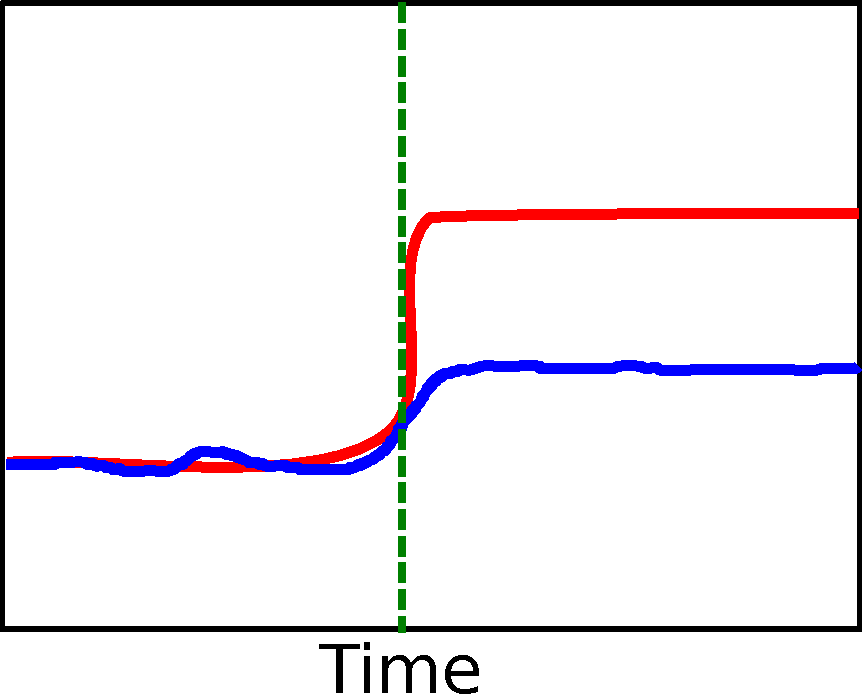
\includegraphics[width=.98\linewidth]{fig/contribPush}
% 		\caption{\textbf{\nameref{sec:results:exp1}:} Tracking error. After the contact with the obstacle (\textcolor{darkgreen}{dark vertical line}) the error for the standard inverse dynamics grow (\textcolor{red}{red}) while with our learned model the contribution remains limited.}
% 		\label{fig:pusherror}
% 	\end{figure}
%     %
    
%     %
%     \begin{figure}[t]
% 		\centering
% 		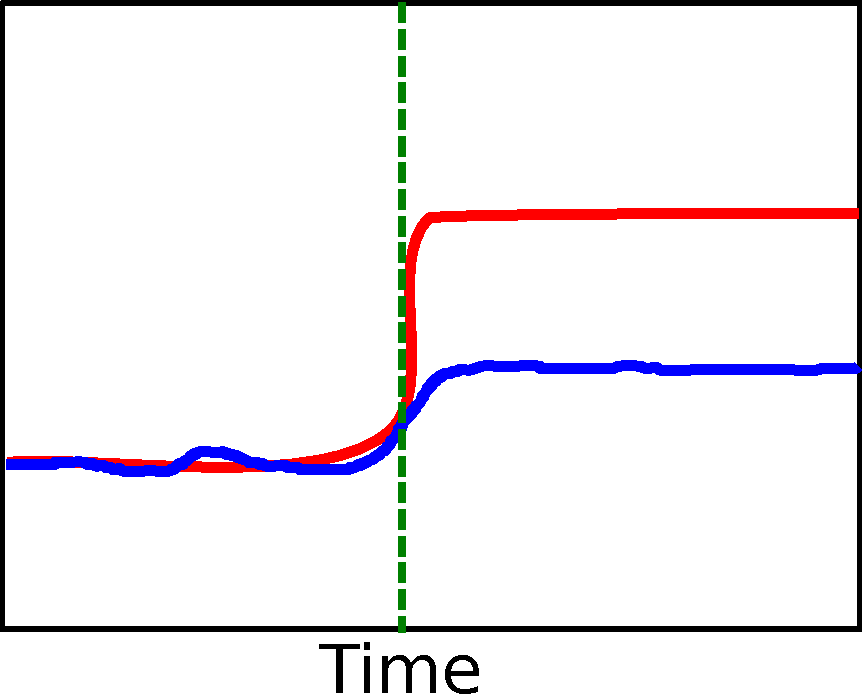
\includegraphics[width=.98\linewidth]{fig/contribPush}
% 		\caption{\textbf{\nameref{sec:results:exp1}:} Analysis of the contribution from the PD controller. After the contact with the obstacle (\textcolor{darkgreen}{dark vertical line}) the contribution for the standard inverse dynamics grow (\textcolor{red}{red}) while with our learned model the contribution remains limited. This result }
% 		\label{fig:pushcontroller}
% 	\end{figure}
%     %



%===============================================================================

%\subsection{Sliding Along Obstacles}
%\label{sec:results:exp2}
%
%	%
%    \begin{wrapfigure}{r}{0.2\columnwidth}
%	%\begin{figure}[t]
%		\centering
%		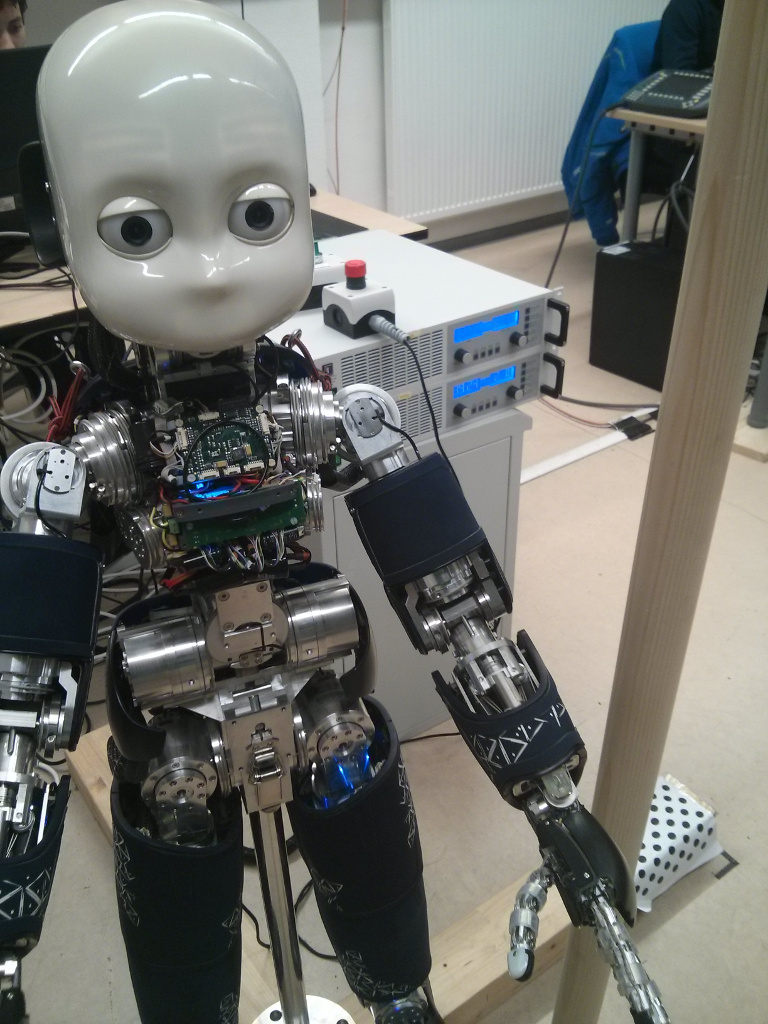
\includegraphics[width=.98\linewidth]{robertoIROS/fig/taskSlide}
%		\caption{\textbf{\nameref{sec:results:exp2}.}}
%		\label{fig:slideSetup}
%	%\end{figure}
%    \end{wrapfigure}
%	%
%
%	The goal of this second scenario is to control the robot in order to slide along an obstruction. 


% 	%
% 	\begin{figure}[t]
% 		\centering
%         \begin{subfigure}[t]{0.45\hsize}
% 			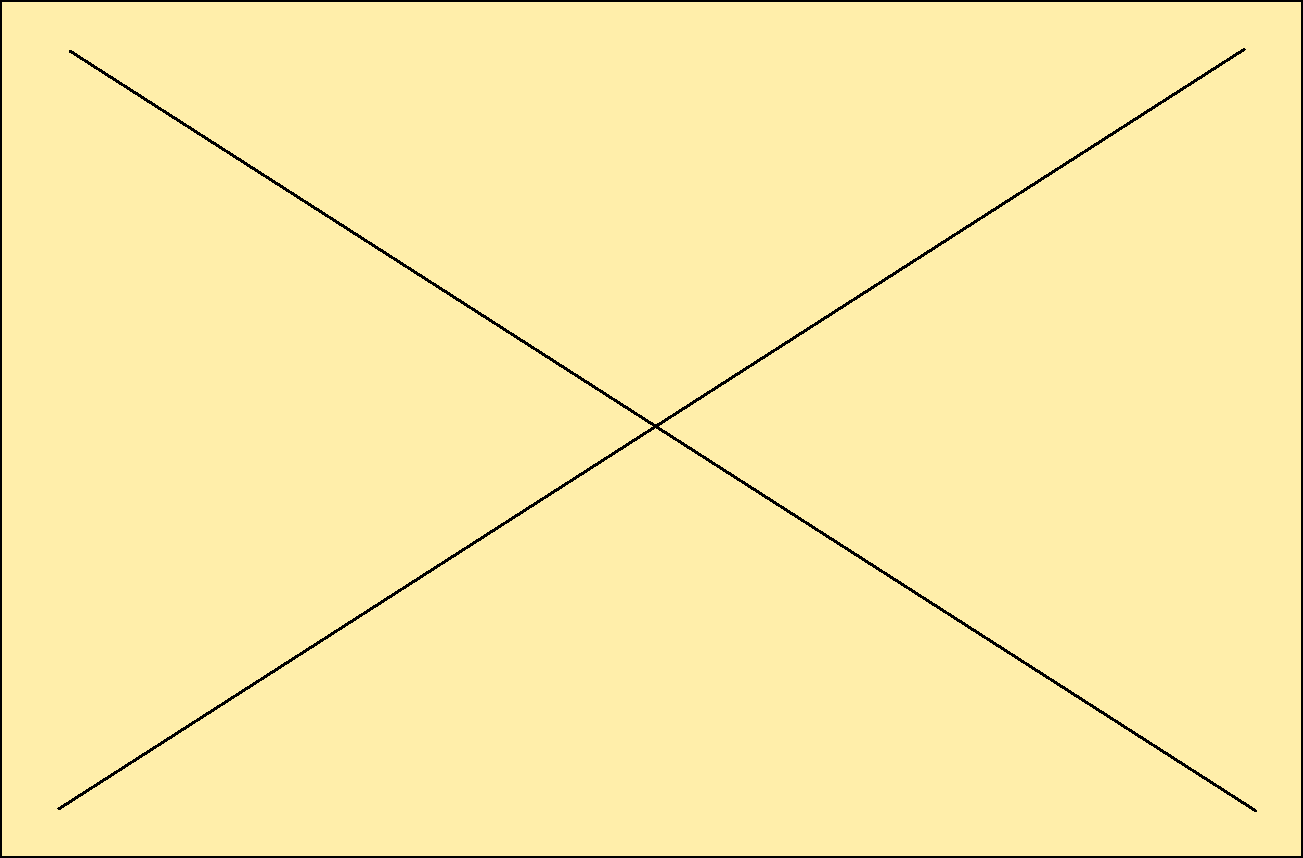
\includegraphics[width=.98\columnwidth]{fig/empty}
%             \caption{With obstacle}
%         \end{subfigure}
%         \hfill
% 		\begin{subfigure}[t]{0.45\hsize}
%         	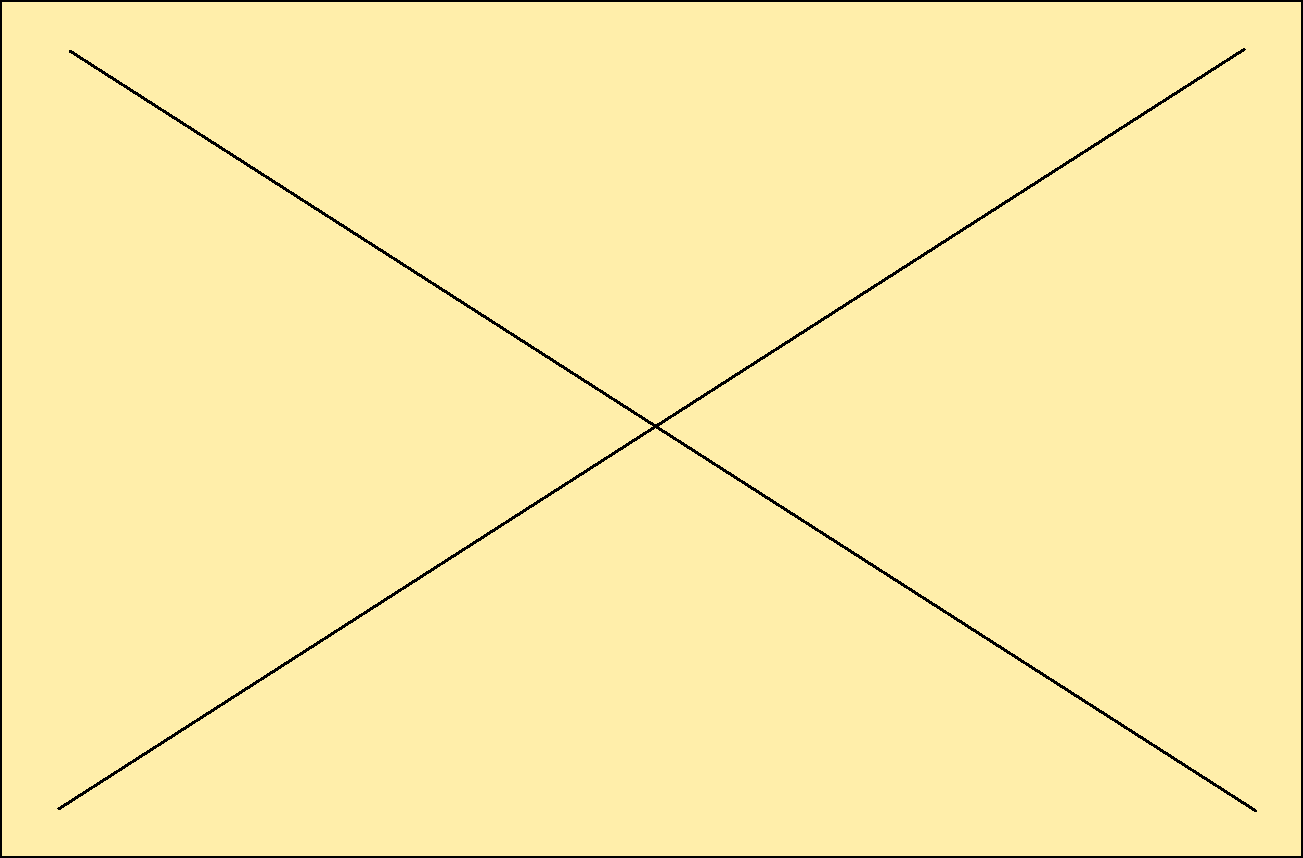
\includegraphics[width=.98\columnwidth]{fig/empty}
%             \caption{Without obstacle}
%         \end{subfigure}
        
% 		\caption{\textbf{\nameref{sec:results:exp2}:} Trajectory of the end effector with and without obstacle.}
% 		\label{fig:slideTraj}
% 	\end{figure}
% 	%


%===============================================================================
